% !TeX spellcheck = ru_RU_yo
% !TEX program = xelatex

\documentclass[pta]{../../scs-iam}

\begin{document}

\newgeometry{
  top=20mm,
  right=15mm,
  bottom=20mm,
  left=20mm,
  bindingoffset=0cm
}

\thispagestyle{empty}

\begin{center}
  {
    \bfseries
    {
      \subnormal
      Министерство образования и науки Российской Федерации
    } \\[-0.5em]
    {
      \scriptsize
      ФЕДЕРАЛЬНОЕ ГОСУДАРСТВЕННОЕ АВТОНОМНОЕ ОБРАЗОВАТЕЛЬНОЕ УЧРЕЖДЕНИЕ ВЫСШЕГО ОБРАЗОВАНИЯ
    } \\[-0.25em]
    {
      \subnormal
      “САНКТ-ПЕТЕРБУРГСКИЙ НАЦИОНАЛЬНЫЙ ИССЛЕДОВАТЕЛЬСКИЙ \\[-0.5em]
      УНИВЕРСИТЕТ ИНФОРМАЦИОННЫХ ТЕХНОЛОГИЙ, \\[-0.75em]
      МЕХАНИКИ И ОПТИКИ”
    }
  }
\end{center}

\small

\begin{center}
  \vskip -1em
  {
    \bfseries
    {
      \large
      ОТЗЫВ РЕЦЕНЗЕНТА \\
    }
    О  ВЫПУСКНОЙ  КВАЛИФИКАЦИОННОЙ  РАБОТЕ
  }
\end{center}

\vskip -1.25em

{
  \parindent0pt
  
  \textbf{Студент}
  \underline{\text{\strut Кузнецов А.А.~\,}}
  \hfill
  \textbf{Группа}
  \underline{\text{\strut P4215~\,}}
  \hfill
  \textbf{Кафедра}
  \underline{\text{\strut ИПМ~\,}}
  \hfill
  \textbf{Факультет}
  \underline{\text{\strut ПИиКТ~\,}} \\[-1.25em]
  
  \titledline{\textbf{Квалификация}}
  \uline{магистр\hfill} \\[-1.25em]

  \titledline{\textbf{Направление подготовки (специальность)}}
  \uline{09.04.01 -- Информатика и вычислительная техника\hfill} \\[-1.25em]

  \titledline{\textbf{Направленность (профиль)}}
  \uline{09.04.01 -- Математические модели и компьютерное моделирование\hfill} \\[-1.25em]

  \titledline{\textbf{Наименование темы}}
  \uline{Разработка веб-приложения для работы с программным пакетом высоко\-точного позиционирования RTKLIB\hfill} \\[-1.25em]

  \titledline{\textbf{Рецензент}}
  $\underset{
    \text{\scriptsize (Фамилия, И., О., место  работы, должность, ученое звание, степень)}
  }{
    \underline{\makebox[\remaining][s]{\hfill}}
  }$ \\[-1.75em]
}

\begin{center}
  \textbf{ОЦЕНКА ВЫПУСКНОЙ КВАЛИФИКАЦИОННОЙ РАБОТЫ}
\end{center}

\vskip -1.75em

{
  \parindent0pt
  \footnotesize
  
  \begin{figure}[h!]
    \centering
    \setlength{\fboxsep}{0pt}
    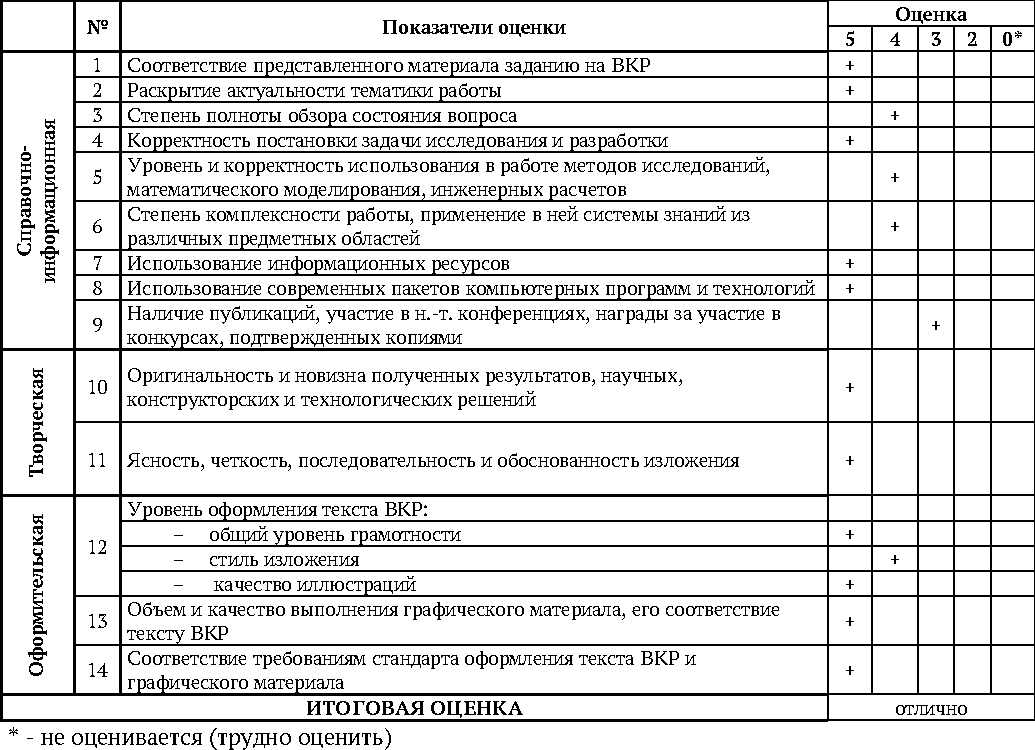
\includegraphics[width=\textwidth]{table}
  \end{figure}
}

\end{document}
